\section{Binning as means of Imaging}
digital imaging from lecture
sampling etc
Binning is a way to find underlying distribution.


\section{SASE fluctuations}
% 2024-08-16-13-56-32.png

Check the dld detector electron copies causing problem

\section{Poisson process checking}

There's a lot of parameters that need to be tested to determine what sort of counting statistics the dataset has.

Controls for the test:
lets see
\begin{itemize}
    \item Total time being looked at (like 1000 s or 20 hours)
    \begin{itemize}
        \item distribution might change due to overtime FEL intensity changes
    \end{itemize}
    \item Time bins being used (like 2 s vs 20 s and so on).
    \begin{itemize}
        \item Seems like distribution changes based on that too
    \end{itemize}
    \item Looking at individual pixels on X and Y
    \item Looking at Energy axis as it behaves weirder
    \item Looking at a larger region in X and Y 
    \begin{itemize}
        \item should follow same statisitics as single pixels
    \end{itemize}
    \item Check after removing correlated electrons within each pulse
    \begin{itemize}
        \item It is possible that electrons are correlated between different pulses because the time delay is long enough. But seems highly unlikely!
    \end{itemize}
    \begin{itemize}
        \item 
    \end{itemize}
\end{itemize}


\subsection{Before filtering}

\begin{figure}
    \centering
    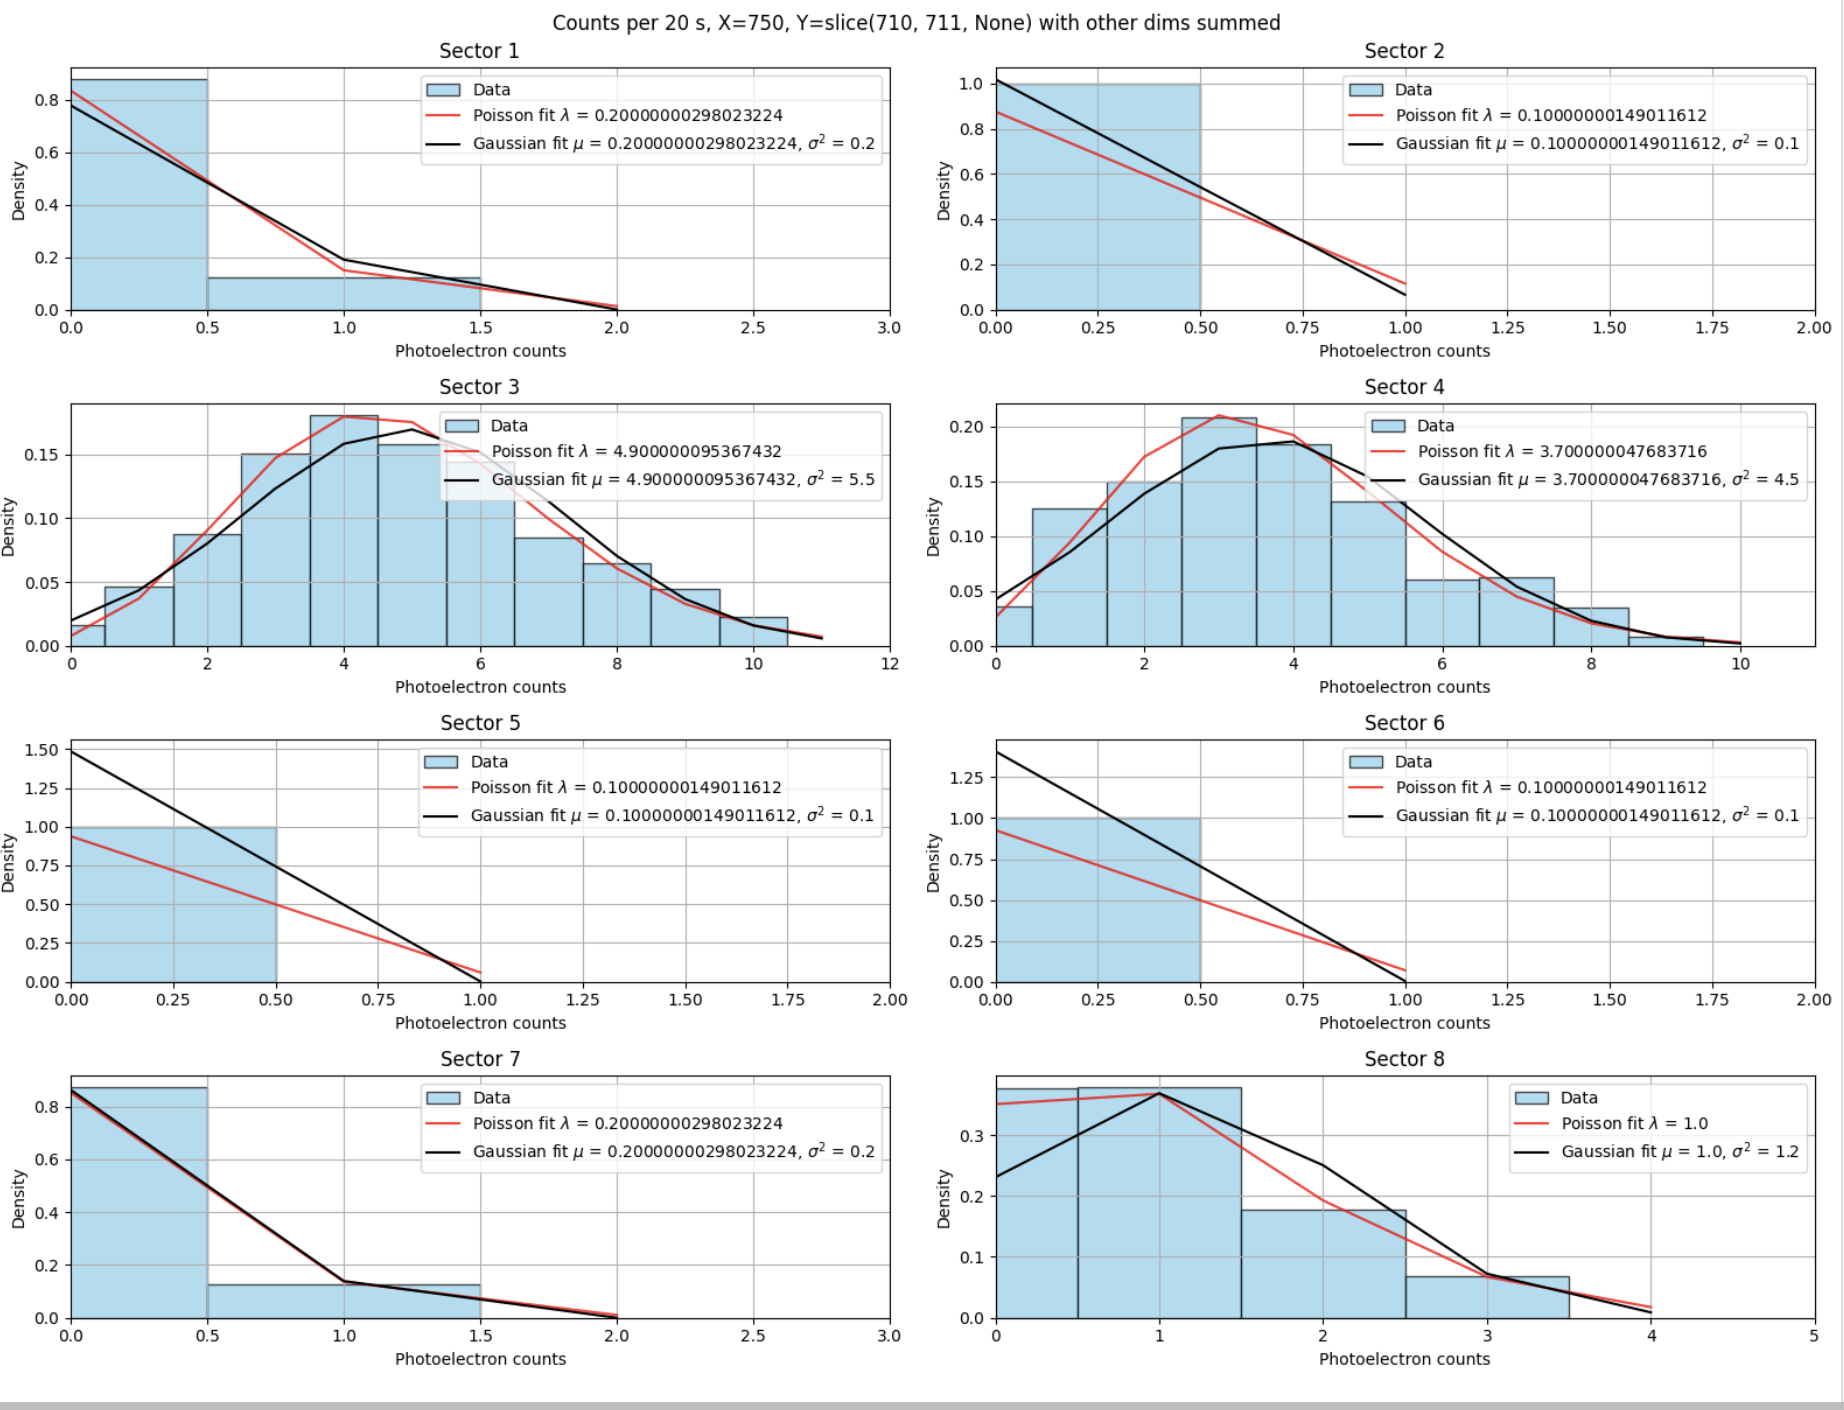
\includegraphics[width=1\linewidth]{images/image.png}
    \caption{Enter Caption}
    \label{Image at one 2D pixel but summed over energy}
\end{figure}

\begin{figure}
    \centering
    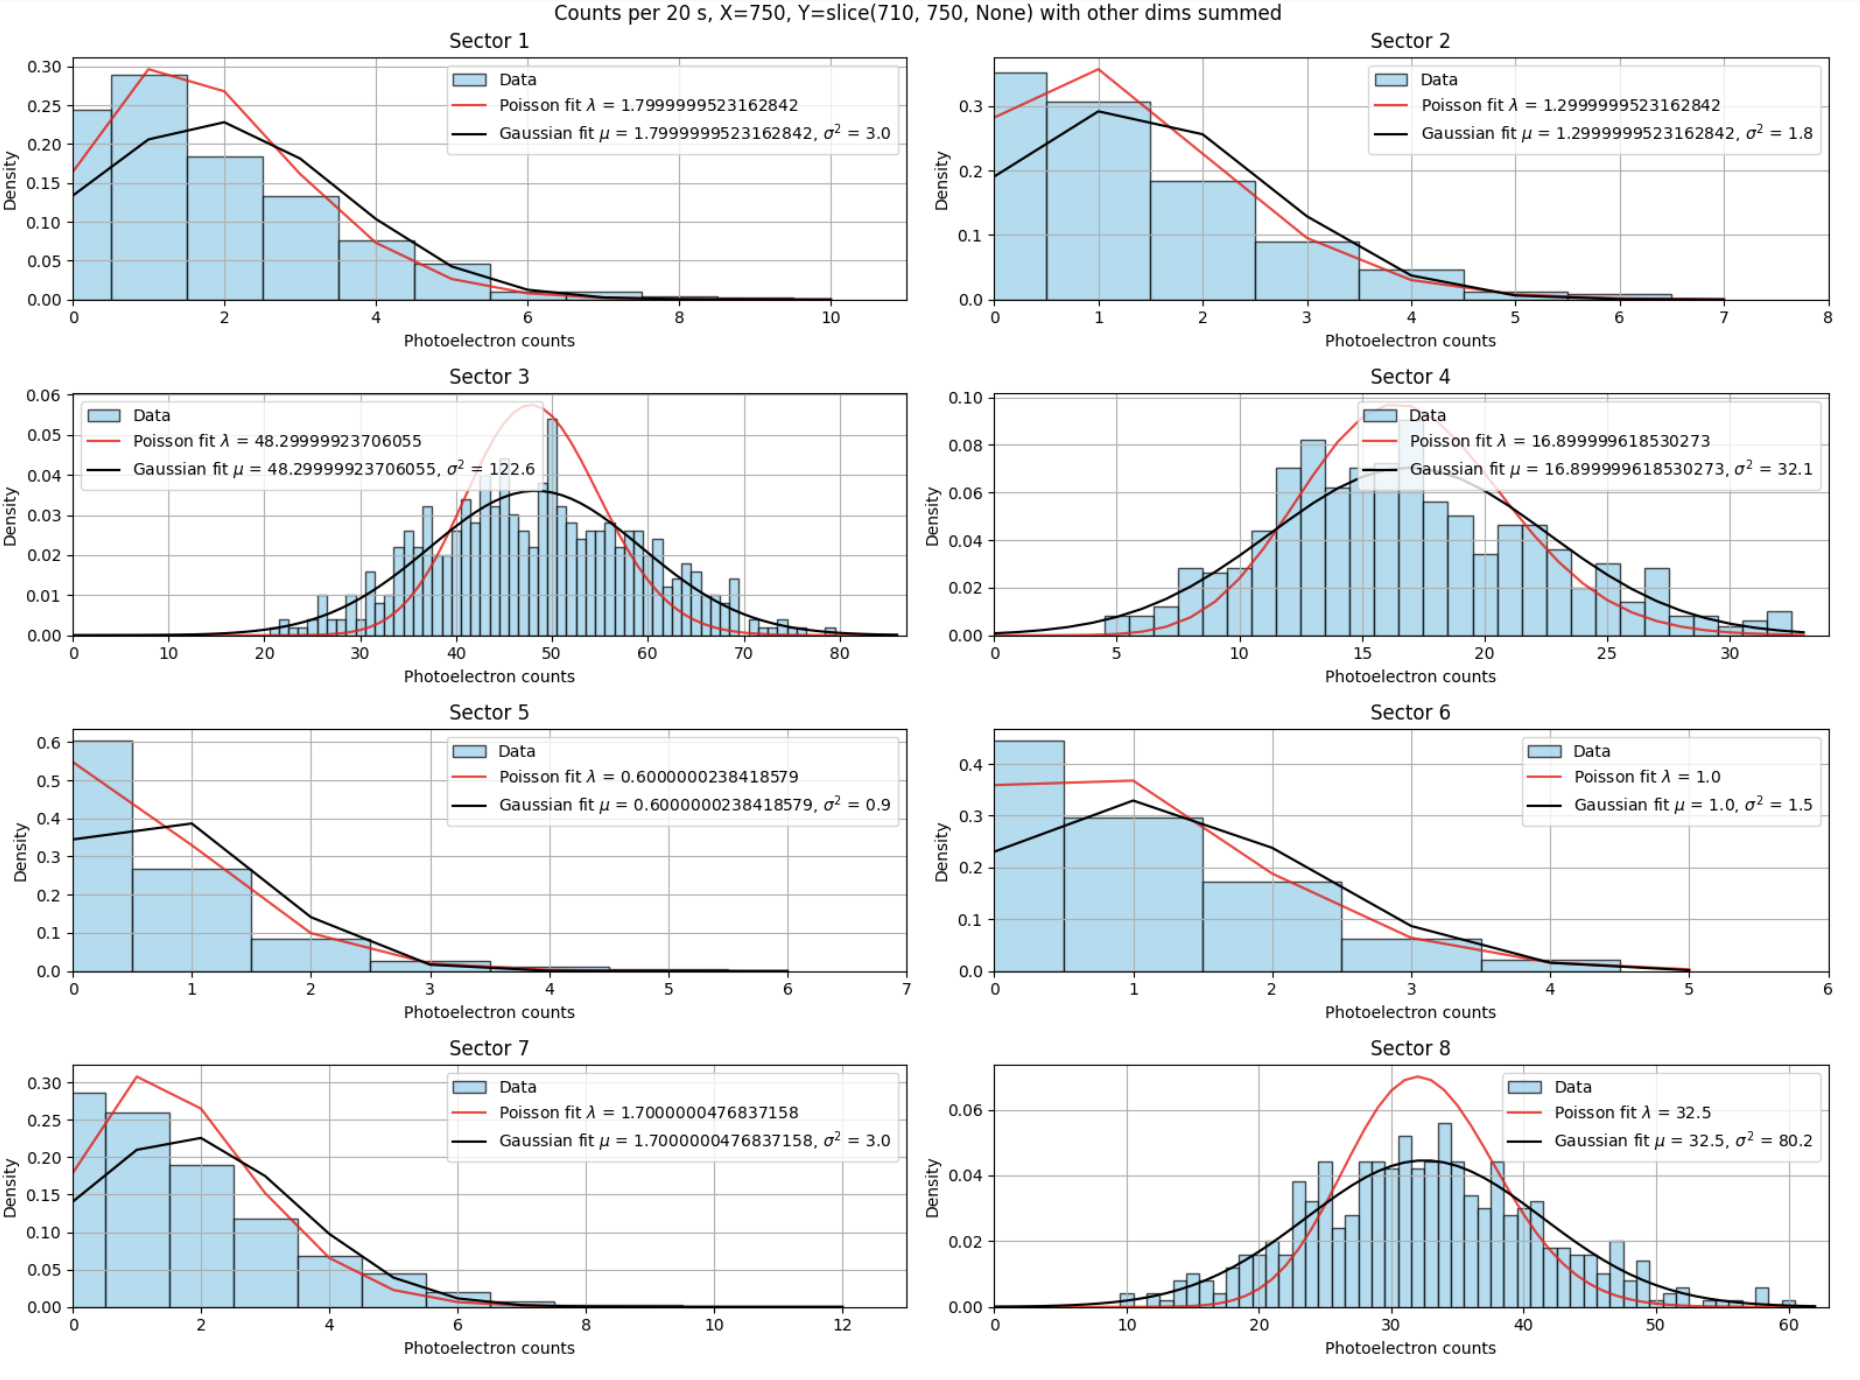
\includegraphics[width=1\linewidth]{images/summed.png}
    \caption{Image over 40 pixels and summed over energy}
    % \label{fig:enter-label}
\end{figure}

\subsection{After filtering}

\begin{figure}
    \centering
    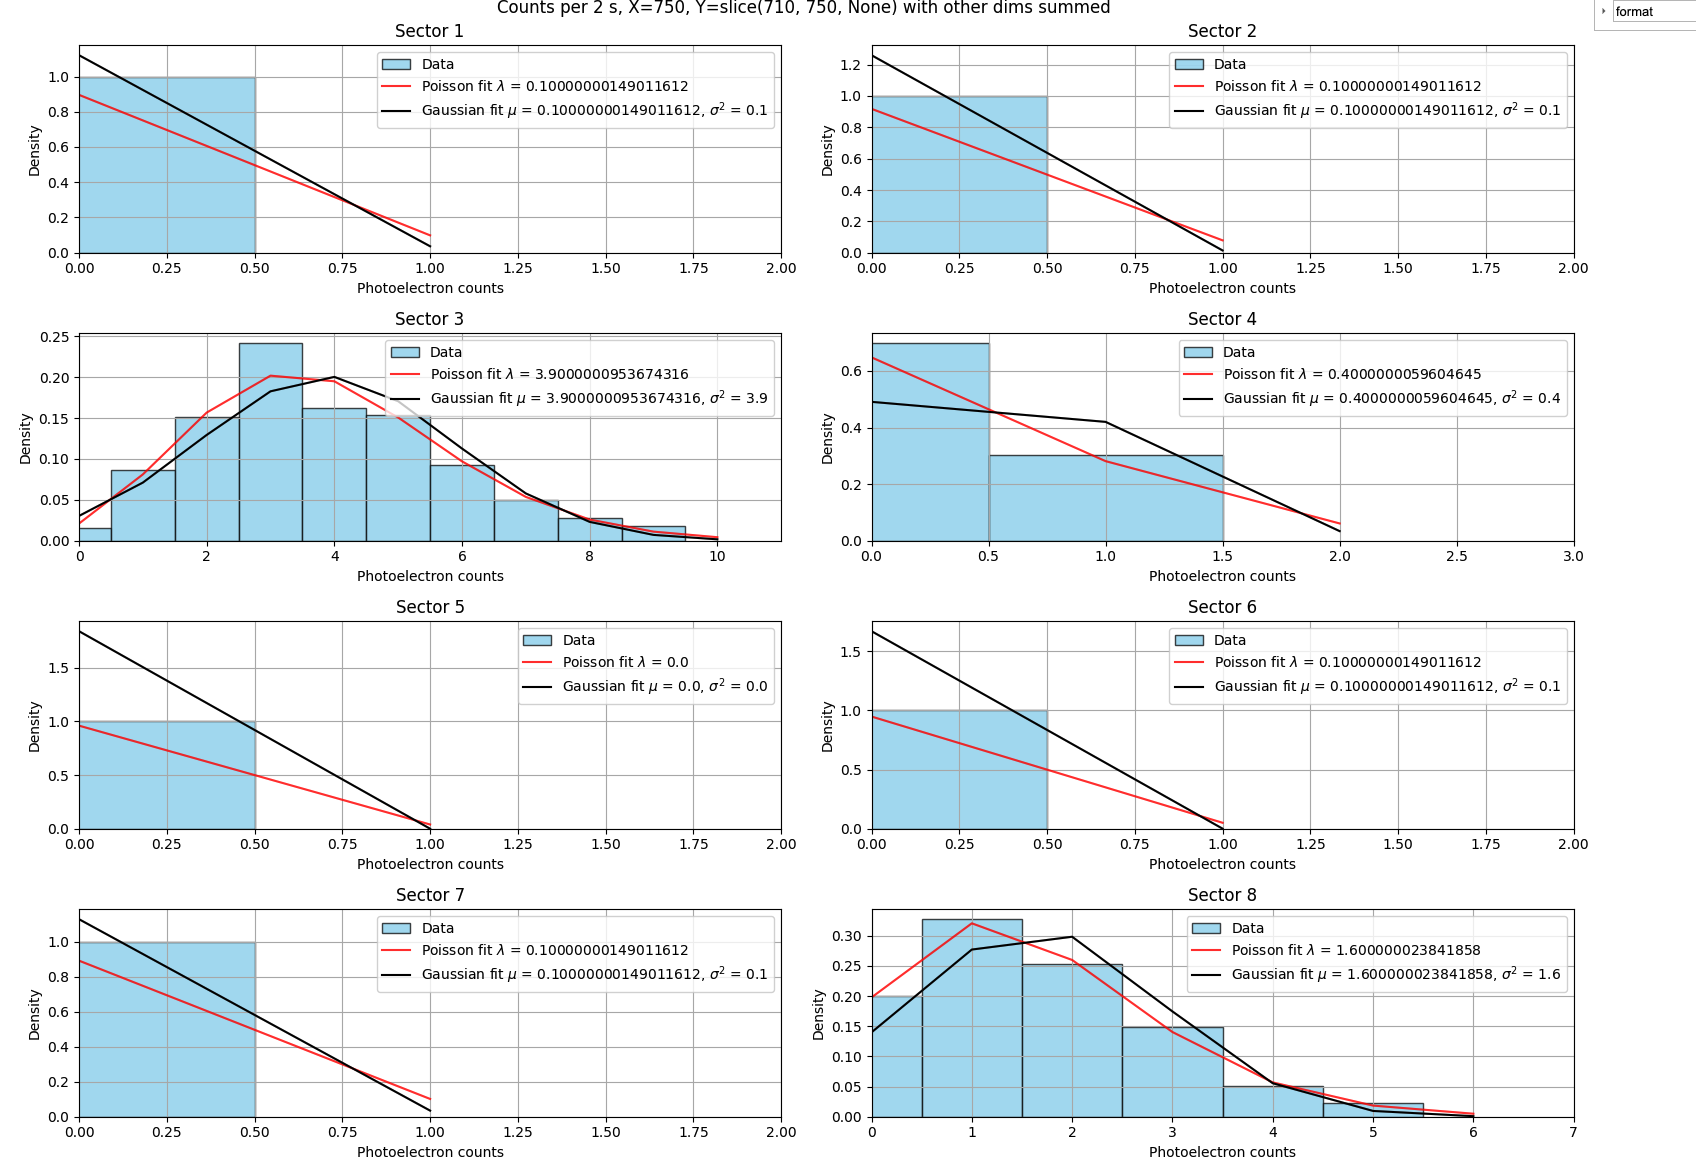
\includegraphics[width=1\linewidth]{images/poisson_stats/after_filtering_region_1000s.png}
    \caption{Data is filtered here with the KNN and looking at small region}
    % \label{fig:enter-label}
\end{figure}

\begin{figure}
    \centering
    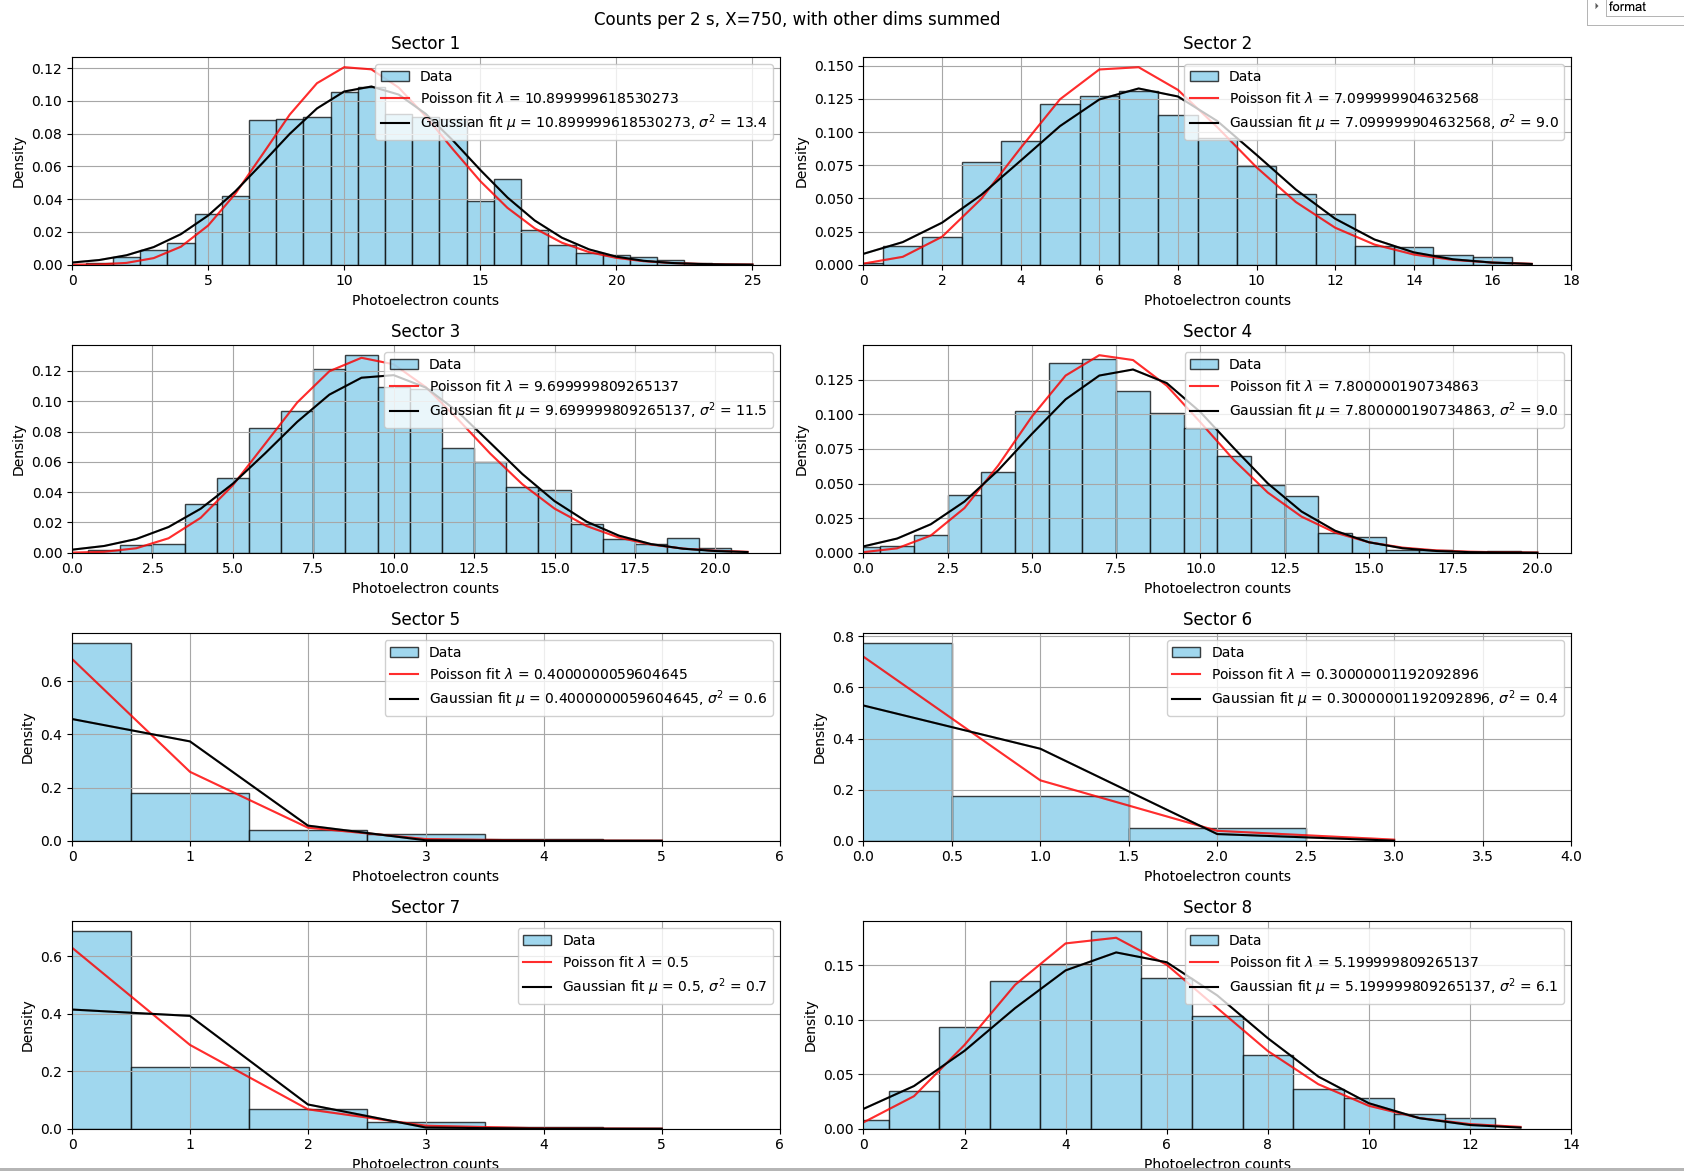
\includegraphics[width=1\linewidth]{images/poisson_stats/filtered_allY_singleX.png}
    \caption{Enter Caption}
    % \label{fig:enter-label}
\end{figure}


